\documentclass[titlepage,a4paper]{jsarticle}
\usepackage{../../sty/import}%各種パッケージインポート
\usepackage{../../sty/title_team}%タイトルページの変更
% レポートタイトル
\title{球体-木製ブロック衝突実験の\\重回帰分析を用いた分析}
% 提出日
\expdate{\today}                      
% 科目名
\subject{情報システム工学実験}          
% 分野  
\class{情報経営システム工学分野}          
% 学年 
\grade{B3}                
% 学籍番号             
\mynumber{24336488}
% 記述者
\author{本間三暉}
% グループ名
\team{10}
\begin{document}
\maketitle
\section{はじめに}
% 本実験の目的や行ったことを記述
\subsection{前置き}
今回の実験で物理実験を行うに当たり,16班に分かれ,各班ごとに実験を行い実験結果をExcelにまとめた.
その実験結果を一つにまとめる際ラベル等の指定がなかったため,おおよそデータの分析を行うとは思えないような形式でまとめている班が散見された.

そのため,各班に呼びかけ形式の統一を行うよう呼びかけた.
しかし,現時点(2024年6月27日)で,形式の統一が行われておらずどの数字が実験データかわからない班が3班,単位が正しく直されていなさそうな班が1班いた.

そのような数字はデータの前処理の段階で排除したため,16班分のデータを用いた想定通りのデータ分析が行えないことを断っておきたい.
また,形式を統一した際に,平均値のみを提出した班と生データを提出した班があるため,データの数に偏りがあることも断っておきたい.

\subsection{目的}
現代社会において,データサイエンスの重要性はますます高まっている.
データサイエンスとは,与えられたデータに基づいて知見を見出し,その知見を次の行動に活かすことを目的としている.
本レポートでは,データ分析の基本的な手法とその応用について実験を通じて探求する.

本実験は,データ分析の5つの手順(PPDACサイクル)に基づいて進められる.
PPDACサイクルは,問題の把握(Problem),調査の計画(Plan),データの収集(Data),データの分析(Analysis),および結論の考(Conclusion)
の5つのステップから成り立つ.
これらのステップを踏むことで,データから有用な情報を引き出し,具体的な課題解決に繋げることを目指す.

本レポートの目的は,実験を通じてデータ分析の基本的な手法を理解し,実際のデータを用いた分析のプロセスを経験することである.
さらに,得られた知見をもとに具体的な解決策を提案し,実務に応用できるスキルを身につけることを目指す.

\section{データ(実験概要)}
% どのような実験装置でどういったデータを取ったかを記述
% 他の球体とブロックを使った実験データは,他のグループのデータを採用する.
今回の実験では,図\ref{class}のような装置を用いて行う.
\begin{figure}[H]
  \centering
  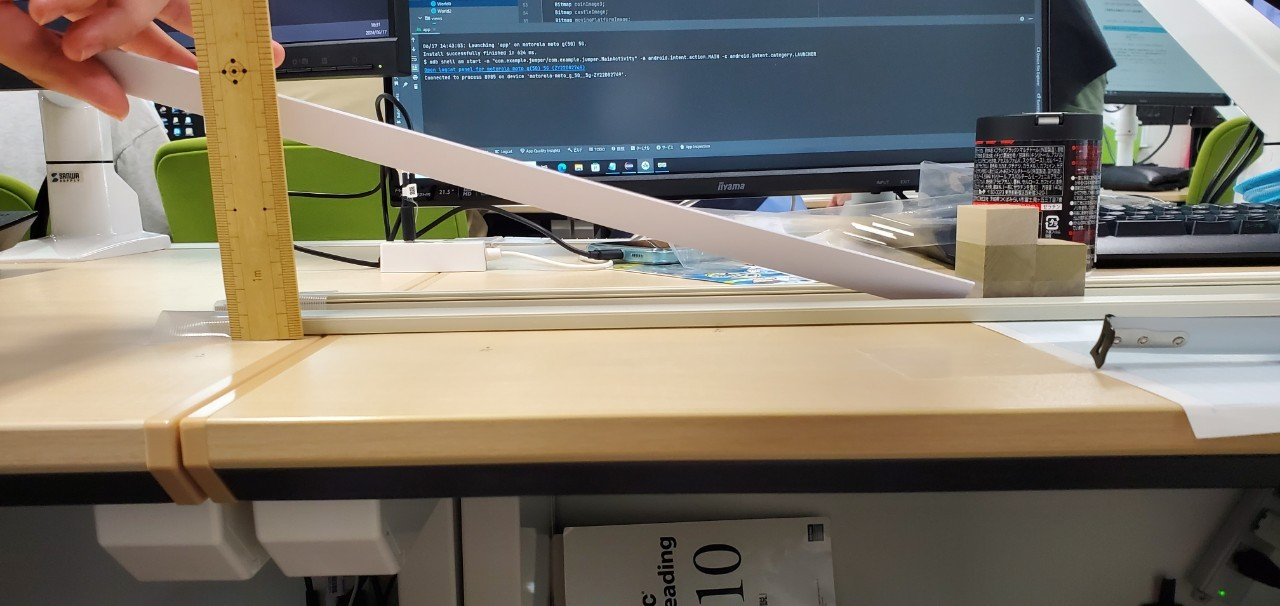
\includegraphics[width=12cm]{img/data_science1.jpg}
  \caption{実験装置}
  \label{class}
\end{figure}
今回,私の班はボールが転がり始める高さ(以下高さ),地面と平行な向きのボールの転がる距離(以下底辺),物体の移動距離(以下移動距離)を測定し,
ボールが転がる距離(以下斜辺),斜辺と底辺のなす角(角度)などは計算で導出することにした.
斜辺の導出方法は,斜辺を$C$,高さを$A$,底辺を$B$とした時,三平方の定理から式\eqref{Pythagoras}で導出できる.
\begin{align}
  C^{2} & = A^{2} + B^{2}                           \\
  C     & = \sqrt{A^{2} + B^{2}} \label{Pythagoras}
\end{align}
また,角度は測定値である高さと底辺から導出する.
高さを$A$,底辺を$B$,角度を$\theta$とした時,タンジェントの定義式から,アークタンジェントを用いた式\eqref{atan}から導出できる.
\begin{align}
  \tan \theta & = \frac{A}{B}                                   \\
  \theta      & = \arctan \left(\frac{A}{B}\right) \label{atan}
\end{align}
Excelの関数ATAN()は戻り値の単位がラジアンなので,これを度数法に直す必要がある.
弧度法は,扇形を考えた時,中心角$\theta$は円弧の長さ$l$に比例する.
円弧の長さ$l$と扇型の半径$r$の比をとると,同じ角度$\theta$に対して扇型の大きさにかかわらずこの比は一定である.
という性質を利用して角度の大きさを式\eqref{rad}を用いて定義されている.
\begin{align}
  \theta & = \frac{l}{r}\label{rad}
\end{align}
よって弧度法から度数法に変換するためには,弧度法の角度を$\theta$,度数法の角度を$\theta'$とした時,式\eqref{conbert}を用いれば良い.
\begin{align}
  \theta' & = \frac{360}{2\pi}\theta \label{conbert}
\end{align}


\section{データの前処理}
% 前処理で行ったことを記述
\subsection{グループデータ}
% ・グループデータ
\subsection{統合データ}
% ・全グループ統合データ

\section{相関分析・単回帰分析}
\subsection{相関分析}
\subsection{単回帰分析}

\section{重回帰分析}
\subsection{グループデータ}
% ・球体・ブロック各1種のグループデータで行った重回帰分析について記述
%  説明変数の選択方法
%  重回帰式
%  修正済決定係数とあてはまりのよさを記述
% P 値と説明力について記述
% ※余裕があれば未計測の説明変数値での計算予測値と実測値の比較をしてみる

\section{全グループデータ}
% ・全グループデータを合わせた重回帰分析について記述
%  説明変数の選択方法
%  重回帰式
%  修正済決定係数とあてはまりのよさを記述
% P 値と説明力について記述
% ※余裕があれば未計測の組み合わせ等での計算予測値と実測値の比較をしてみる

\section{おわりに}
\subsection{結論}
% 本分析の結論として考えられる特徴を記述
\subsection{考察}
% 木製ブロックの移動距離に影響する要素は~等
\subsection{反省点}
% 反省点:球体の種類のデータ数に偏りがあった.全種類バランスよくデータを取れるように実験計画を見直す必要がある.
\subsection{要望}
% テンプレートの統一等について,来年以降の学生に向けて欠点をお願いすること
\end{document}